% Also note that the "draftcls" or "draftclsnofoot", not "draft", option
% should be used if it is desired that the figures are to be displayed in
% draft mode.
%
\documentclass[conference,a4paper]{IEEEtran}

%\usepackage[latin1]{inputenc} % Latin1
\usepackage[utf8]{inputenc} 	% UTF-8
\usepackage[T1]{fontenc}
\usepackage{microtype}
\usepackage{amsmath}
\usepackage{amssymb}
\usepackage{amsfonts}
%\usepackage{breeq}
\usepackage[pdftex]{graphicx}
%\graphicspath{{./figures/}}
\newcommand{\e}[1]{{\mathbb E}\left[ #1 \right]}
\newcommand{\p}{P}
%\DeclareGraphicsExtensions{.pdf}
\usepackage{siunitx}

% Metadata
\usepackage[final=true]{hyperref}
\hypersetup{
	pdfauthor = {Ankit Kaushik et al.},
	pdftitle = {ISWCS, Ilmenau 2013},
	pdfsubject = {ISWCS, Ilmenau 2013},
%	hidelinks = {true}
}
\title{Cognitive Relay: Detecting Spectrum Holes in a Dynamic Scenario}
\IEEEspecialpapernotice{(Extended Abstract)}
\author{Ankit Kaushik, Marcus Mueller, Friedrich K. Jondral \\
        Communications Engineering Lab, Karlsruhe Institute of Technology (KIT) \\
        \{\href{mailto:Ankit.Kaushik@kit.edu}{Ankit.Kaushik}, 
        \href{mailto:Friedrich.Jondral@kit.edu}{Friedrich.Jondral}\}@kit.edu,
        \href{mailto:Marcus.Mueller@student.kit.edu}{Marcus.Mueller@student.kit.edu} }
\begin{document}
%
% make the title area
\maketitle
\thispagestyle{empty}
\pagestyle{empty}
%\begin{abstract}
%4 lines.... \\
%4 lines.... \\
%4 lines.... \\
%4 lines....
%\end{abstract}
%%%%%%%%%%%%%%%%%%%%%%%%%%%%%%%%%%%%%%%%%%%%%%%%%%%%%%%%%%%%%%%%%%%%%%%%%%%%%%%%%%%%%%%%%
\section{Introduction}
%%%%%%%%%%%%%%%%%%%%%%%%%%%%%%%%%%%%%%%%%%%%%%%%%%%%%%%%%%%%%%%%%%%%%%%%%%%%%%%%%%%%%%%%%
Cognitive radio as first coined by Mitola \cite{mitola} in 1999 illustrates a
dynamic model that provides human intervention to the underlying radio
hardware.
Dynamic spectrum access (DSA) is one of the many applications of
cognitive radio. The DSA umbrella \cite{QS07} considers the secondary usage of
the spectrum. On these grounds, we meant to design a working prototype for
Cognitive Relay (CR), a device that dynamically accesses the spectrum to
support wireless services operating indoor.\\
Through the concept of CR the authors
attempt to bring the basic aspects of the cognition cycle: \textit{sensing} and
\textit{learning} using real hardware. The concept of dynamic access is
accomplished through a cross layer optimization. The information gathered
through sensing and the intelligent access to the spectrum have already been
considered in literature \cite{hossain09}.

Yet there have been limitations: Firstly, in many cases the physical parameters and protocols are
specific to the underlying standards.
Secondly, due to the complexity involved,
the time required to implement these concepts is large. To overcome these
problems the CR considers a general architecture for sensing and a basic
algorithm for scheduling the resources. This paper discusses the implementation
of its prototype.

The paper is organized as follows: Section \ref{sec:scenario}
discusses the scenario for the CR. Section \ref{sec:dect} explains the
detection technique and the scheduling algorithm. Section \ref{sec:imple}
describes the implementation of the device. Finally, section \ref{sec:userint}
presents the user interaction of the demonstrator in a real-world scenario followed
by section \ref{sec:conc} which concludes the paper.

%%%%%%%%%%%%%%%%%%%%%%%%%%%%%%%%%%%%%%%%%%%%%%%%%%%%%%%%%%%%%%%%%%%%%%%%%%%%%%%%%%%%%%%%%
\section{Cognitive Relay} \label{sec:scenario}
%%%%%%%%%%%%%%%%%%%%%%%%%%%%%%%%%%%%%%%%%%%%%%%%%%%%%%%%%%%%%%%%%%%%%%%%%%%%%%%%%%%%%%%%%
\begin{figure}[!t]
	\centering
	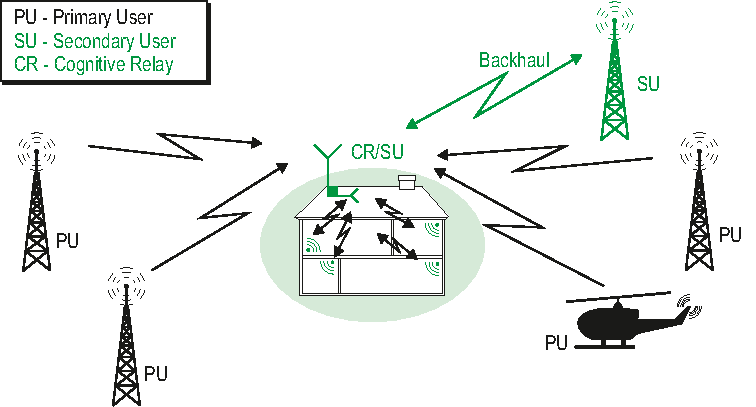
\includegraphics[scale=.62]{figures/wo_channels_CR_Scenario_farbig}
	\caption{A scenario demonstrating the interaction between the PU and the CR. The CR senses PU operating on different channels the outdoor to provide a dynamic access to the devices operating indoor.}
	\label{fig:scenario}
\end{figure}
Fig.~\ref{fig:scenario} depicts a scenario for the CR. It
is a network element that belongs to the mobile network operator (MNO), who
aims to access the spectrum as a Secondary User (SU) when it is not used by the
Primary User (PU). Through the deployment of CR in an indoor environment,
the MNO can improve its networks' capacity by optimizing spectral efficiency.
The CR has an \textit{outdoor antenna}
that is situated at an elevated position and an
\textit{indoor antenna} that communicates with the user equipment (UE)
registered for indoor usage.

The \textit{backhaul link} between the SU and CR
is directional. This simplifies the channel and reduces the transmitted power
both at the CR and the SU.

By nature of their access, the PUs leave temporal and spatial gaps in the spectrum termed as \textit{Spectrum Holes} \cite{Weiss}.
The CR enables dynamic access to the spectrum and utilization of these spectrum holes.
The biggest challenge for the cognitive radio devices acting as SUs is to avoid interference at the primary receiver while accessing the PU spectrum.
%%%%%%%%%%%%%%%%%%%%%%%%%%%%%%%%%%%%%%%%%%%%%%%%%%%%%%%%%%%%%%%%%%%%%%%%%%%%%%%%%%%%%%%%%
\section{Detection and Learning} \label{sec:dect} 
%%%%%%%%%%%%%%%%%%%%%%%%%%%%%%%%%%%%%%%%%%%%%%%%%%%%%%%%%%%%%%%%%%%%%%%%%%%%%%%%
We consider the receiver model $Y[n] = X[n] + W[n]$, 
representing the signal at the receiver $Y[n]$ in terms of input signal $X[n]$ with additive white Gaussian noise $W[n]$. 
Following the Neyman Pearson approach, the CR uses a binary hypothesis $\mathcal{H}_0$, $\mathcal{H}_1$ to determine the absence
of PUs ($W[n]$) or their presence ($X[n]+W[n]$).
Energy detection \cite{Urkowitz} is used to decide upon the hypothesis.
The test statistic
\begin{equation}\label{eq:Hypo}
T(\textbf{Y}) = \frac{1}{K} \sum\limits_{n=0}^{K-1} |Y[n]|^2 \mathop{\gtrless}_{\mathcal{H}_1}^{\mathcal{H}_0} \gamma
\end{equation}
corresponds to the energy of the $K$ complex input samples.
For large $K$, $T(\textbf{Y})$ fulfills the requirements of the 
Central Limit Theorem and follows a Gaussian distribution for the given
hypothesis.

With signal power $\sigma_X^{2}$ as  unknown parameter, a
constant false alarm rate scheme is applied to determine the threshold
$\gamma$. Usually, the PU's spectrum has a wide bandwidth.
The CR employs multiband sensing to retrieve the spectrum occupancy information.
As a result, the CR divides the PU spectrum into subchannels and scans each individual
subchannel by tuning the RF hardware parameters through a software interface.

In the next phase, the binary values for each subchannel are utilized to implement a scheduling algorithm. 
\begin{figure}[!t]
	\centering
	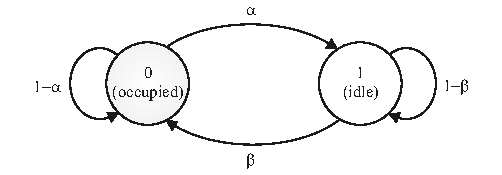
\includegraphics{figures/Markov_channel_mod2}
	\caption{Channel model illustrating the PU access.}
	\label{fig:ChannelModel}
\end{figure}
Through this algorithm, the CR ranks the scanned subchannels.
Following the ranking, a search order is found that minimizes the latency of
finding a suitable subchannel for data transmission.
The CR considers the PU as realizing slotted medium access, the subchannels as independent from each other and the
slots for each subchannel as following the Gilbert channel model \cite{Gilbert}. 

$Z^i(k) = 1$ represents an idle state, while $Z^i(k) = 0$ describes channel $i$ being
occupied at time $k$.
Fig.~\ref{fig:ChannelModel} depicts the slots following a discrete time Markov
process with transitional probabilities $(\alpha, \beta)$. 
The utilization probability $u$ is defined as the probability of finding a channel in occupied state $Z^i(k) = 0$.
Using the given channel model and knowledge of the transition probabilities $(\alpha, \beta)$, $u$ can be evaluated as
\begin{equation} 
        u = \frac{\alpha}{\alpha + \beta} \text{~.}
\label{eq:chauti2}
\end{equation}
While sensing consecutive slots, the CR estimates $(\widehat{\alpha}, \widehat{\beta})$
using Maximum Likelihood Estimation (MLE) \cite{Long}. After
obtaining $u$ for the subchannels, the CR ranks the subchannels and optimizes
its transmission capacity.
%%%%%%%%%%%%%%%%%%%%%%%%%%%%%%%%%%%%%%%%%%%%%%%%%%%%%%%%%%%%%%%%%%%%%%%%%%%%%%%%%%%%%%%%%
\section{Implementation} \label{sec:imple} 
%%%%%%%%%%%%%%%%%%%%%%%%%%%%%%%%%%%%%%%%%%%%%%%%%%%%%%%%%%%%%%%%%%%%%%%%%%%%%%%%
The CR or demonstrator maintains a scanning list inside its database. The
list consists of the PU subchannels to be used for secondary usage over the
indoor link.
For the demonstration GSM subchannels are used, however the
demonstrator can be configured for any other PU architecture that realizes slotted
medium access.

The demonstrator does a live scan of the individual subchannels
in the list. The energy of the input samples is compared 
to $\gamma$ to derive the binary values $z^i(k)$.
The binary values for the individual subchannels are stored in the database.
The channel model parameters
$(\widehat{\alpha^i}, \widehat{\beta^i})$ are estimated for each subchannel.
The demonstrator then determines the $u^i$ for each subchannel over the past observed $1000$ slots.

The hardware of the demonstrator is realized using a calibrated Ettus Research USRP N210, a
software defined radio (SDR) frontend.
The baseband signal processing, the Gilbert channel
modelling and the tuning of RF parameters are done using a general processing unit running
GNU~Radio.
%%%%%%%%%%%%%%%%%%%%%%%%%%%%%%%%%%%%%%%%%%%%%%%%%%%%%%%%%%%%%%%%%%%%%%%%%%%%%%%%%%%%%%%%%
\section{User Interaction} \label{sec:userint}
%%%%%%%%%%%%%%%%%%%%%%%%%%%%%%%%%%%%%%%%%%%%%%%%%%%%%%%%%%%%%%%%%%%%%%%%%%%%%%%%%%%%%%%%%
The demonstrator works in a real-world scenario by monitoring the GSM bands at
\SI{1800}{MHz}.
The spectrum holes in subchannels are  displayed through a
spectrogram, see the snapshot in Fig.~\ref{fig:uti}.
Simultaneously the bar plot shows the subchannels' utilization probability $u^i$
to inform about the ranking of individual subchannels.
The demonstrator updates the plots upon each complete scan. 
%\begin{figure}[!t]
%	\centering
%	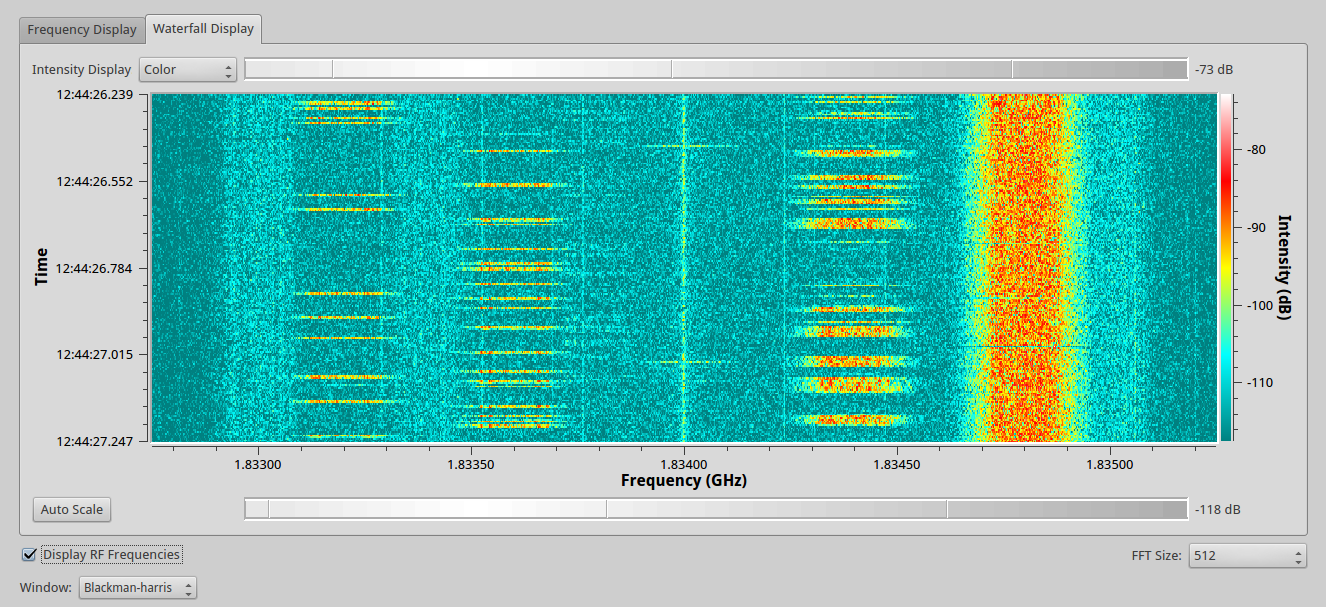
\includegraphics[width=\columnwidth]{figures/ED_GSM}
%	\caption{Energy detection over the \SI{1800}{MHz} GSM subchannels.}
%	\label{fig:ED}
%\end{figure}
%\begin{figure}[!t]
%	\centering
%	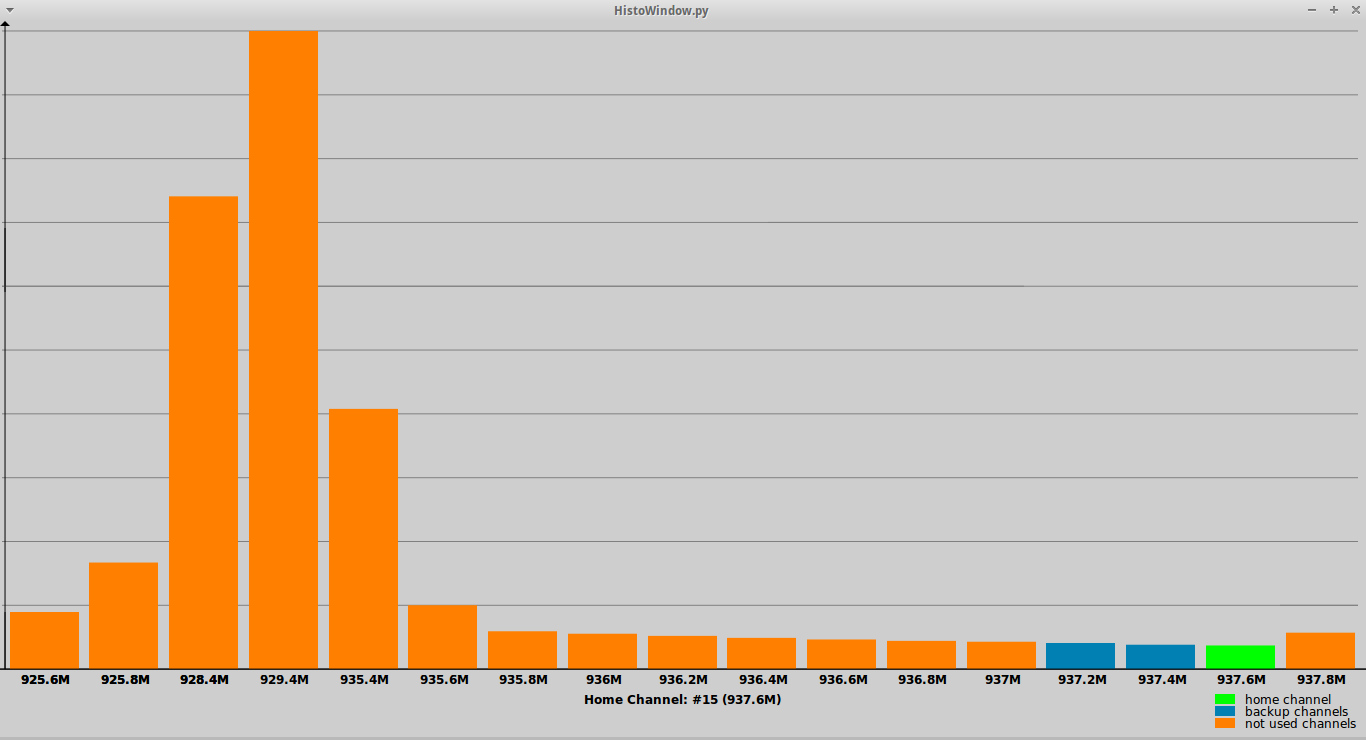
\includegraphics[width=\columnwidth]{figures/UtilizationProbability}
%	\caption{Utilization probability for ranking the GSM subchannels.}
%	\label{fig:uti}
%\end{figure}
%	\label{fig:ED}
%\end{figure}
\begin{figure}[!t]
	\centering
	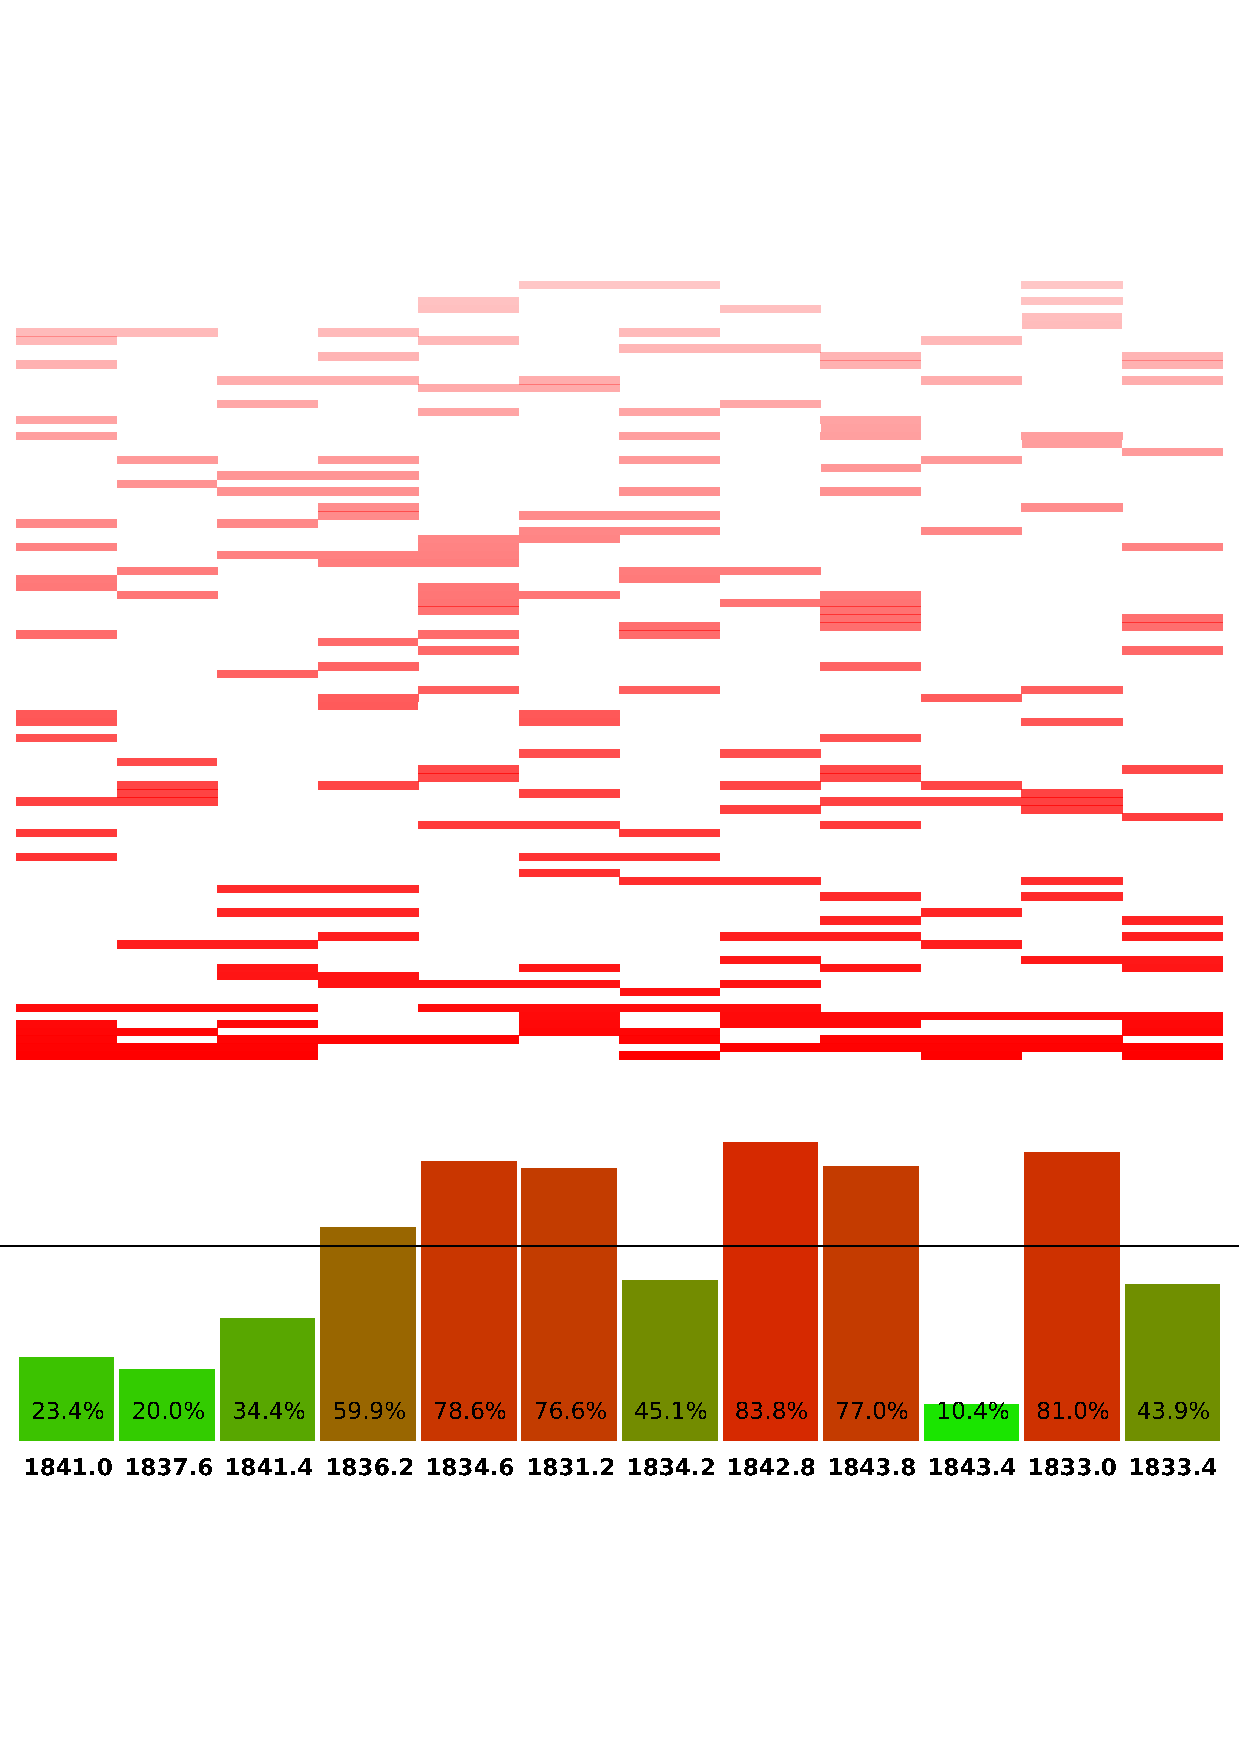
\includegraphics[trim=0.0cm 4.0cm 0.0cm 1.0cm,clip=true,width=\columnwidth]{figures/histo}
	\caption{Utilization probability for ranking the GSM subchannels.}
	\label{fig:uti}
\end{figure}
%\textit{FIXME: One image describing the bar graph for the channel utilization probabilities.}
%%%%%%%%%%%%%%%%%%%%%%%%%%%%%%%%%%%%%%%%%%%%%%%%%%%%%%%%%%%%%%%%%%%%%%%%%%%%%%%%%%%%%%%%%
\section{Conclusion} \label{sec:conc}
%%%%%%%%%%%%%%%%%%%%%%%%%%%%%%%%%%%%%%%%%%%%%%%%%%%%%%%%%%%%%%%%%%%%%%%%%%%%%%%%%%%%%%%%%
The paper considers a demonstration of the Cognitive Relay, a network element
that utilizes the spectrum for secondary usage. It has the potential to sense
and access non contiguous multiple bands and also is capable to learn and
interact with its environment.
%%%%%%%%%%%%%%%%%%%%%%%%%%%%%%%%%%%%%%%%%%%%%%%%%%%%%%%%%%%%%%%%%%%%%%%%%%%%%%%%%%%%%%%%%
%DON'T DELETE THE APPENDIX. IT WILL BE USED LATER
%%%%%%%%%%%%%%%%%%%%%%%%%%%%%%%%%%%%%%%%%%%%%%%%%%%%%%%%%%%%%%%%%%%%%%%%%%%%%%%%%%%%%%%%%
%\section*{Appendix} \label{sec:appendix}
%\subsection*{Noise Calibration}
%The theoretical noise floor is determined using (\ref{eq:theornoisefloor}) is the thermal noise power with added noise figure.
%\begin{equation} \label{eq:theornoisefloor}
%\begin{split}
%\text{Noise floor} &= kTB  + \text{NF} \\
%			  &= -121 + 8\\
%			  &= -115 \text{ dBm} 
%\end{split}
%\end{equation}
%Fig. \ref{fig:USRPCallib} demonstrate the physical interpretation of the digital values in terms of known input power.  
%\begin{figure}[!t]
%	\centering
%	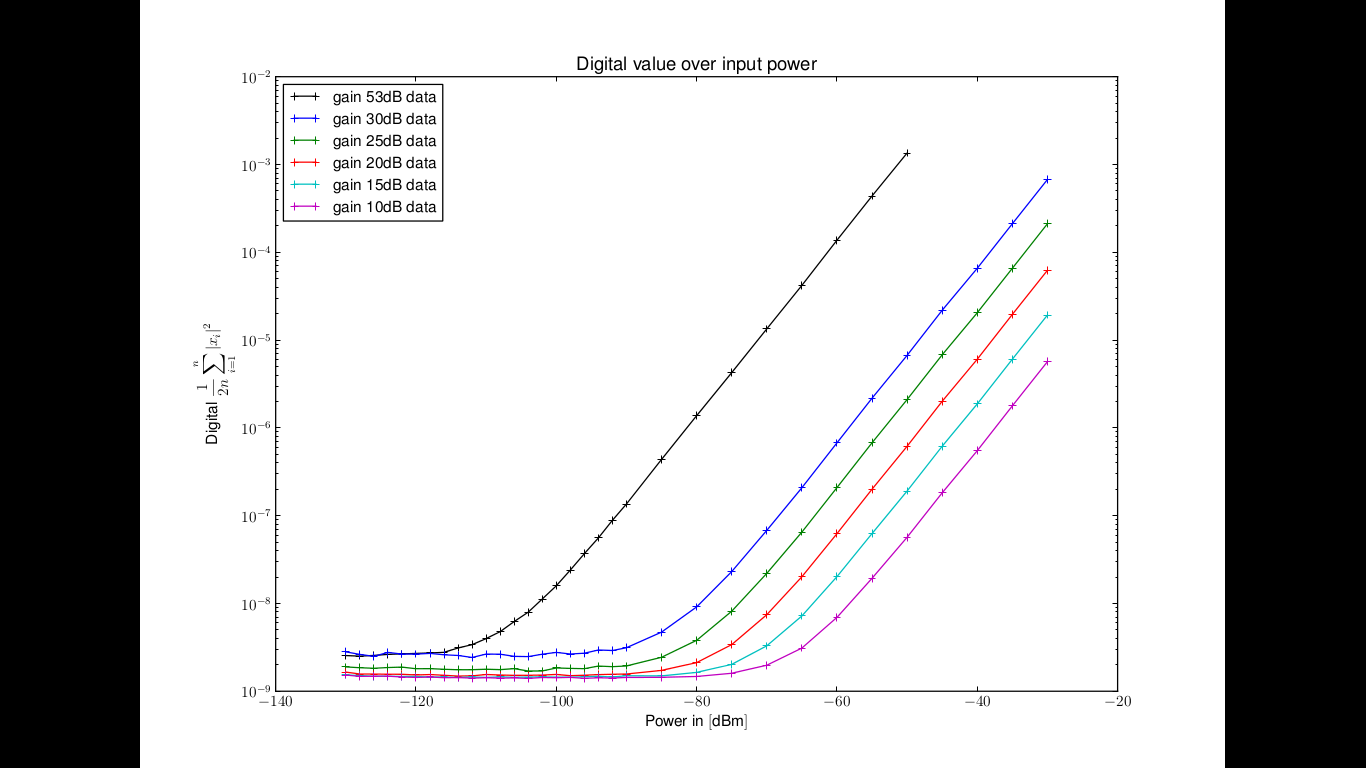
\includegraphics[trim=5.0cm 0.0cm 7.0cm 0.0cm,clip=true,width=\columnwidth]{figures/Callib}
%	\caption{USRP calibration with different gain values.}
%	\label{fig:USRPCallib}
%\end{figure}
%\begin{center}
%	\begin{tabular}{| c | c | c | c |}  
%	\hline
%	Gain 	 	& Th. Noise floor  & Noise Floor & Noise Figure  \\ 
% 	(dB) 	 	& (dBm)			  		 & (dBm)       & (dB) 	      \\ \hline
%	10   	 	& -113 		    		 & -85 		  	 & 26 			  \\ \hline
%	15   	 	& -113 	    			 & -85 		  	 & 26 		 	  \\ \hline
%	20   	 	& -113 	    			 & -95 	   	   & 18 			  \\ \hline
%	25   	 	& -113 	    			 & -95 	 	  	 & 18 		 	  \\ \hline
%	30   	 	& -113 	   	  		 & -95 		     & 18 			  \\ \hline
%	30 + 23 & -119	    			 & -118	       & 3			    \\ \hline
%	\end{tabular}
%\end{center}
%\begin{equation} \label{eq:noisefig}
%\begin{split}
%nf  = nf1 + \frac{(nf2 - 1)}{gain1} 
%\end{split}
%\end{equation}

%%%%%%%%%%%%%%%%%%%%%%%%%%%%%%%%%%%%%%%%%%%%%%%%%%%%%%%%%%%%%%%%%%%%%%%%%%%%%%%%%%%%%%%%%
% References
%%%%%%%%%%%%%%%%%%%%%%%%%%%%%%%%%%%%%%%%%%%%%%%%%%%%%%%%%%%%%%%%%%%%%%%%%%%%%%%%%%%%%%%%%
\bibliographystyle{IEEEtran}
\bibliography{IEEEabrv,refs}
% that's all folks
\end{document}
%Abstract for EADS:
%Cognitive radio has been in discussion for more than a decade. Dynamic access
%to the spectrum is considered its major application to solve the bandwidth demands
%of the mobile network operator. Literature in the form of
%paper and books  exists. Through Cognitive Relaying, the authors make an
%attempt to abridge the gap between the theoretical concepts and a practical
%implementation. 
%Cognitive Relay: Detecting Spectrum Holes in a Dynamic Scenario
%Abstract		
%Cognitive radio has been in discussion for more than a decade. Dynamic access to the spectrum is considered its major application to solve the bandwidth demands of the mobile network operator. Literature in the form of paper and books exists. Through Cognitive Relaying, the authors make an attempt to abridge the gap between the theoretical concepts and a practical implementation.
%Category		 
%Keywords		
%Cognitive radio, dynamic spectrum access
